% !TeX root = ../main.tex

\chapter{绪论}

\section{研究背景和意义}

\subsection{研究背景}
随着目前我国整体经济实力和科研水平的快速上升,计算机视觉技术及其大量成熟的现实应用如图像生成,图像去噪,图像分类等已经凭借着充足的资本支撑,庞大的原料准备和精干的队伍建设在科学和经济领域炙手可热,并对依赖其的下游任务如具身智能,自动驾驶创造了巨大的提升空间和美好前景。
而且随着普通场景下视觉任务的逐渐完善,超越常规硬件的高速运动场景带来的运动模糊,变形,失焦等问题逐渐得到关注。特定领域如航天、军事、体育对高速目标的精准识别提出严格要求。传统的高速相机的工作原理是曝光-读取模式,在一定的时间窗口中通过打开快门使得光感受器接受光子,随后关闭快门进行数据读取。
这个时间窗口就被称之为曝光时间。但这种方式本质上牺牲了连续两张图片之间数据读取时的物体运动,因而会带来不可避免地运动信息丢失。与之相对的,脉冲相机通过异步全时接受光子并进行光电转换,从底层原理上避免了两张图片之间因相机快门的关闭而导致的运动信息丢失。

\begin{figure}[ht]
  \centering
  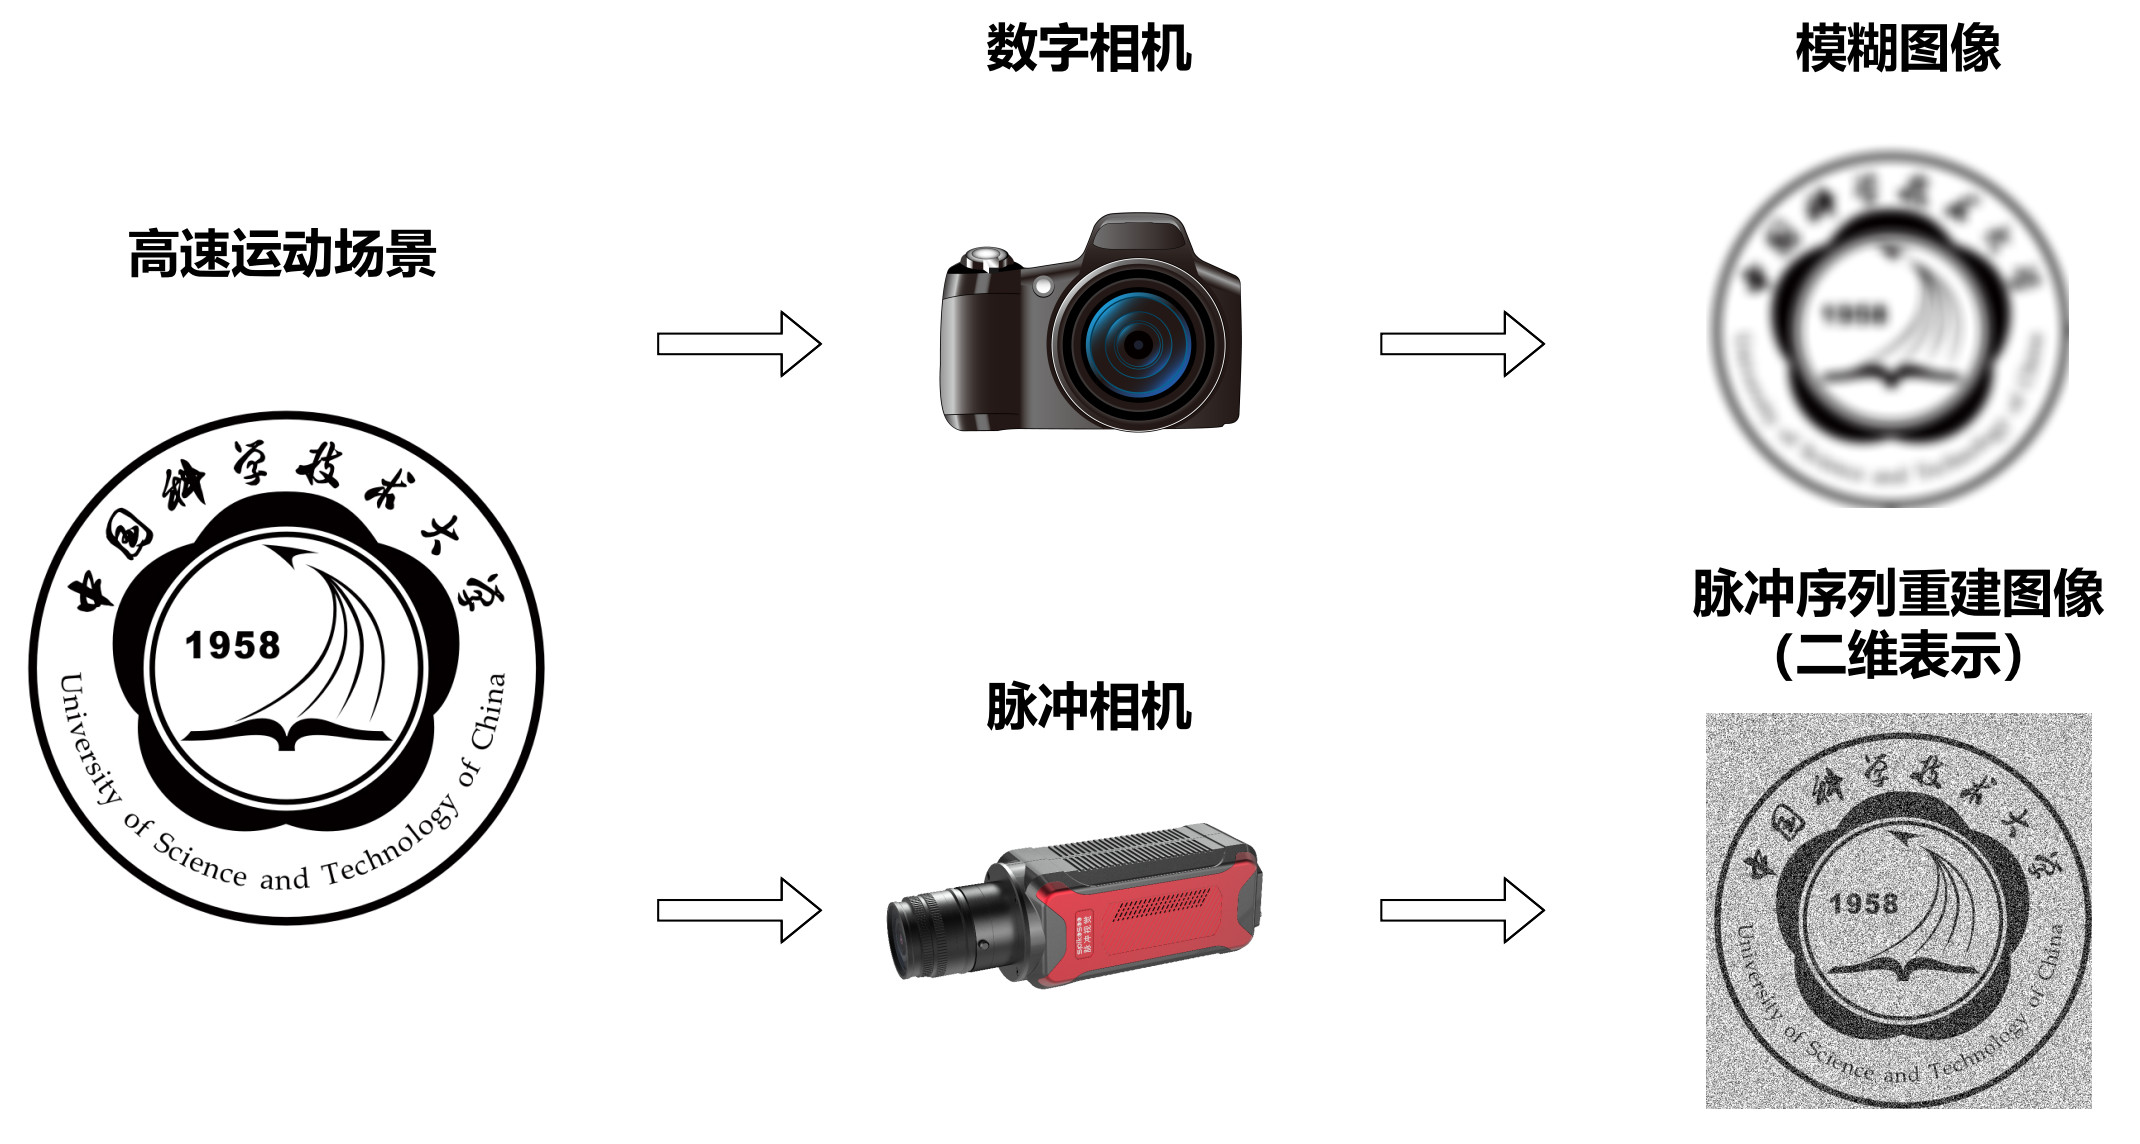
\includegraphics[width=\textwidth]{two_camera_result.jpg}
  \caption{数字相机和脉冲相机对高速运动目标拍摄效果示意图}
  \label{fig:two_camera_result}
\end{figure}    
%这里是插入一张图片的示意
\begin{figure}[ht]
  \centering
  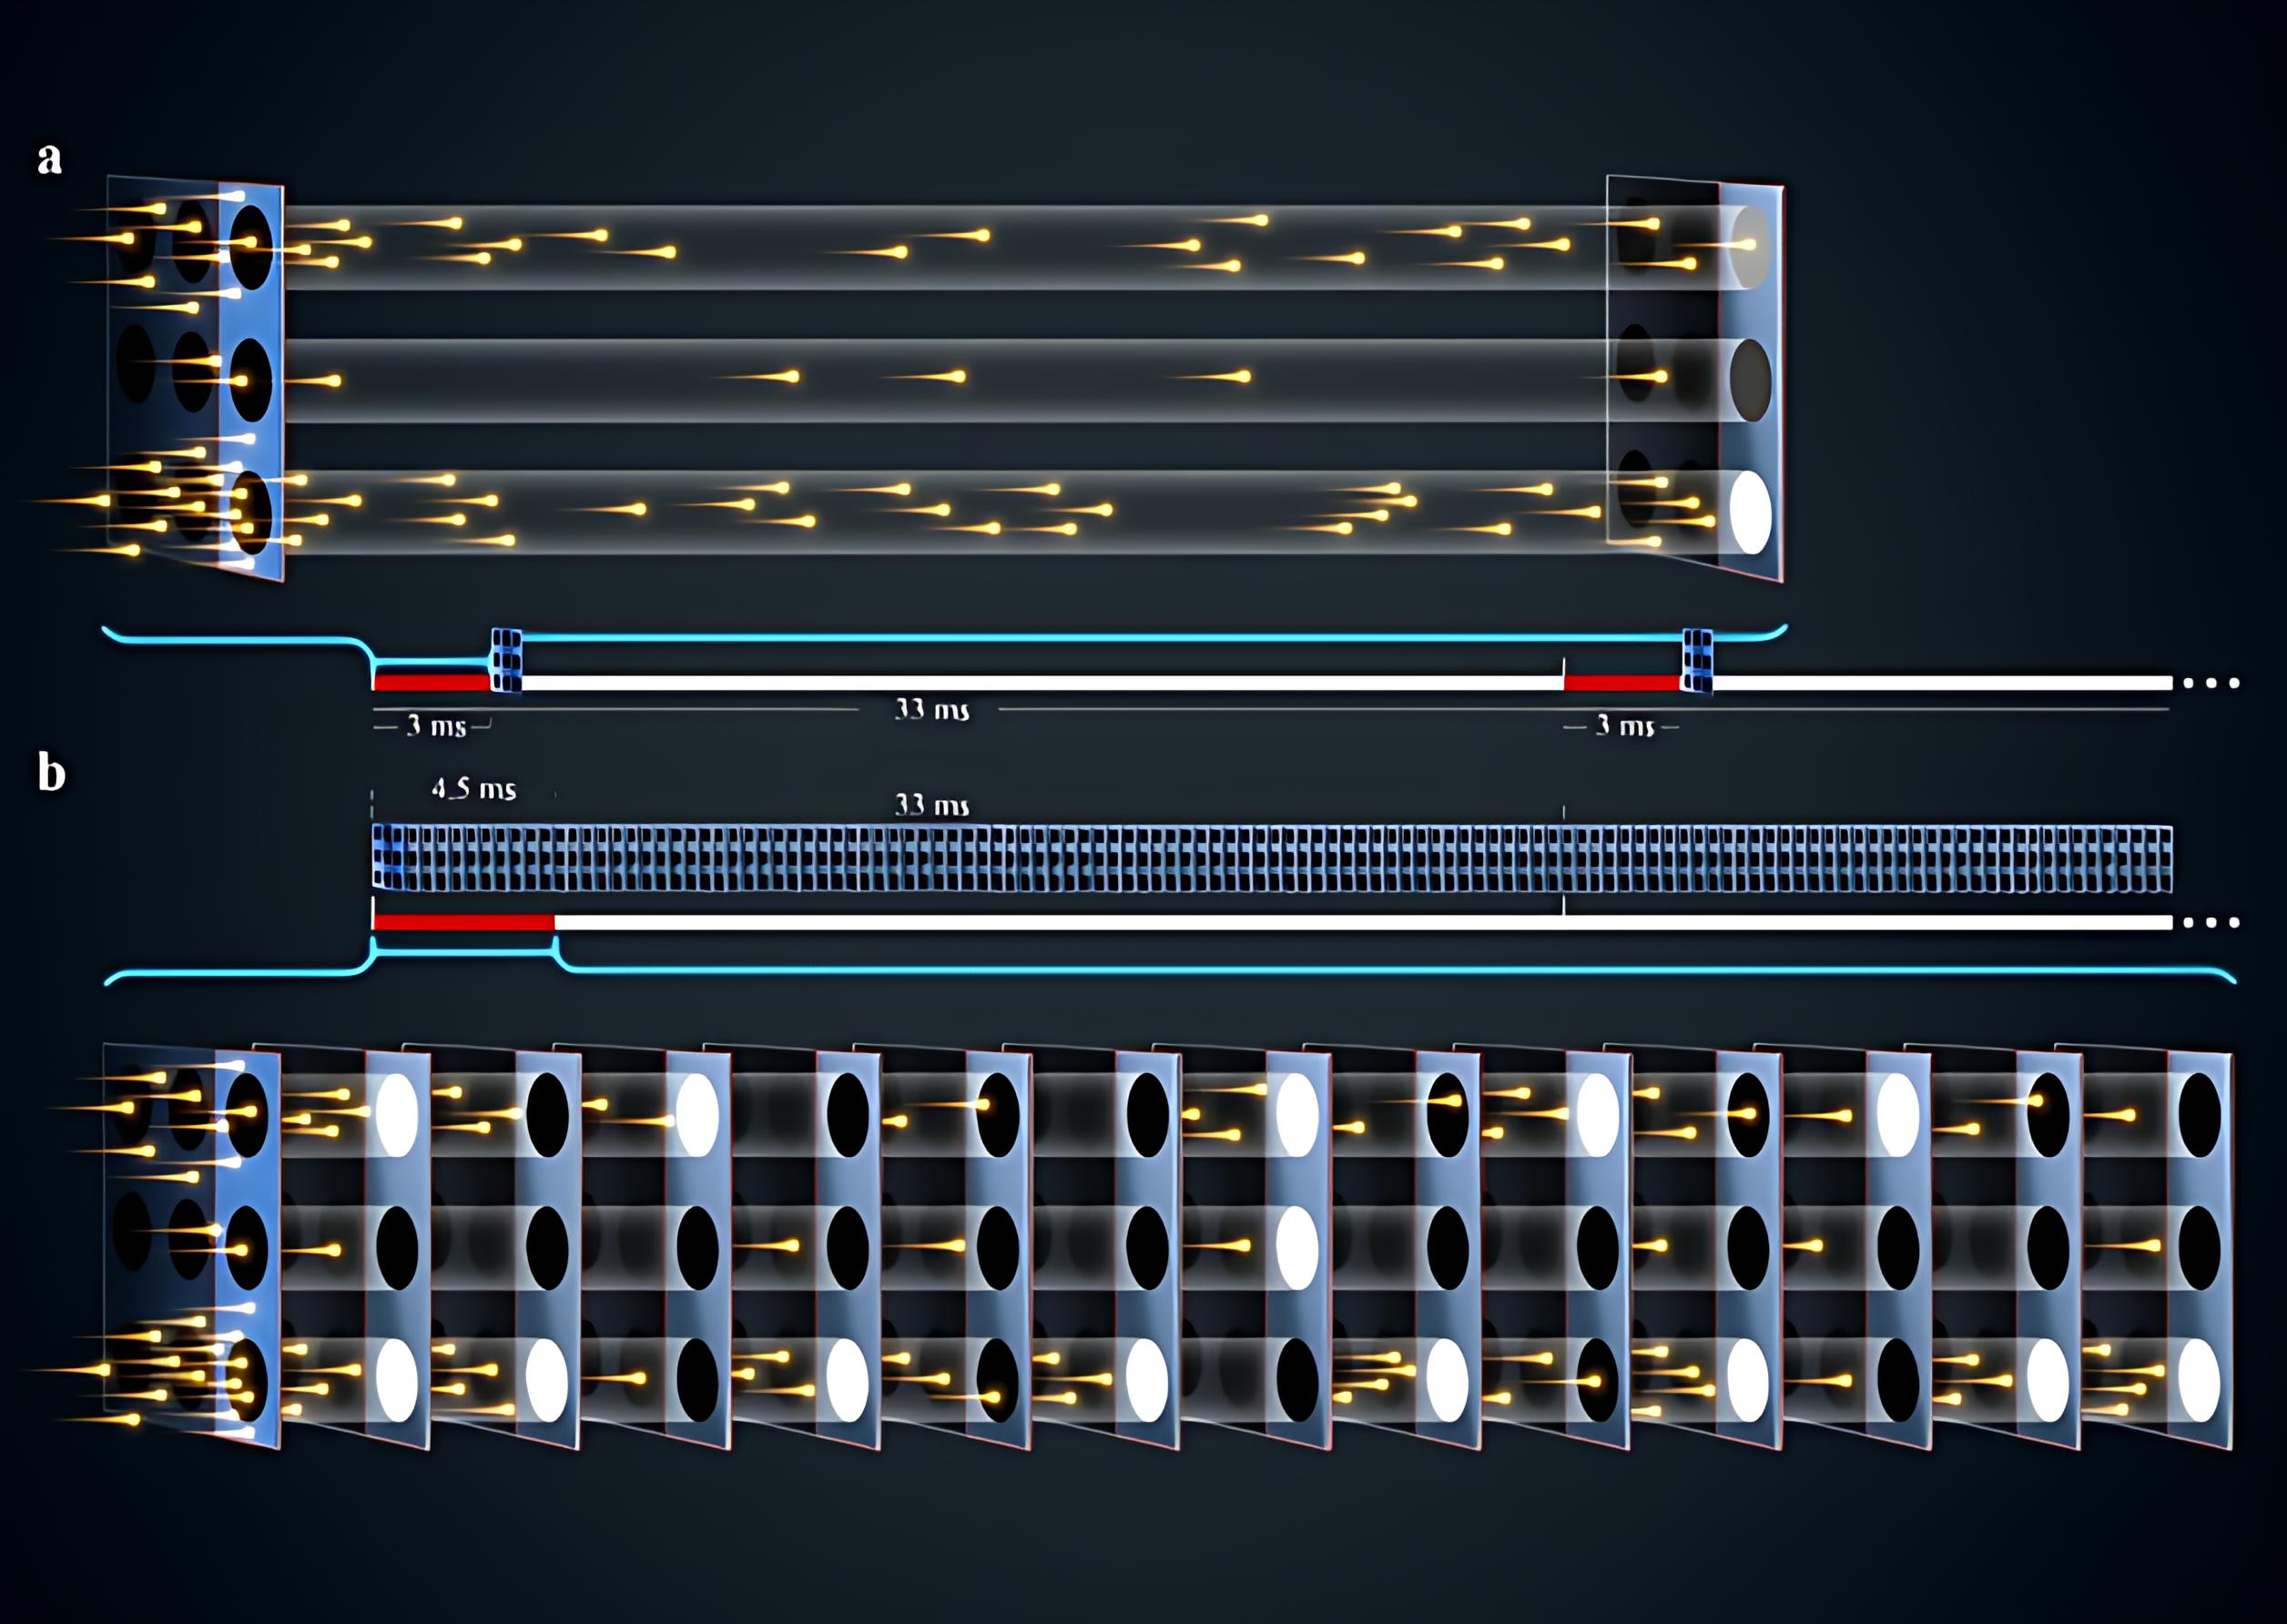
\includegraphics[width=\textwidth]{不同相机成像原理.png}
  \caption{数字曝光成像和脉冲视觉成像在信息获取接受层面的比较}
  \label{fig:two_camera_result_tenet}
\end{figure}    
\subsection{研究意义}
本文初步的研究了脉冲视觉重建和压缩感知理论的结合,通过将压缩感知轻量化、良好解释性等优点应用到脉冲视觉重建中,解决了其他深度学习算法为重复提取特征通过大量卷积带来的模型迅速膨胀和优化了脉冲数据庞大导致传统处理方法时间不敏感的问题,为今后二者结合的其他算法开发提供思路借鉴。同时,在实用领域中,其快速反应的优异特性为未来算法应用到即时快反应场景如自动驾驶、航空航天提供可能。此外,脉冲视觉重建作为上游任务,它的优化可以起到对其他下游任务的普惠作用。


\section{研究问题定义}
\subsection{两种相机成像原理}
“脉冲视觉”是受到灵长类动物视网膜中央凹结构神经回路和其进行信息处理的机制的启发,设计出的有别于传统曝光成像原理的新型视觉表达体系,在成像速度、信息保真率和高速运动捕捉方向都有显著的优势。如图\ref{fig:two_camera_result_tenet}所示,a所代表的传统数字相机在一定时间窗口进行曝光,此时光传感器开始接受光子,随后关闭快门,此时光感受器已经完成了对光子的接受,随后进行光电转换,最后将转换后的图像数据进行读取。下一帧成像重复这个过程。在这个稳定帧率的成像序列中,时刻$t_1$,$t_2$,$t_3$...$t_n$为曝光时刻(时间间隔为$\frac{1}{f}$s),曝光时长是恒定的$\Delta t$($\Delta t$<$\frac{1}{f}$)。将上述所得图像进行顺序排列播放即构成视频,每秒图片排列数量即为视频帧率。于是对于视频而言,上述成像原理带来两帧图片之间($\frac{1}{f}-\Delta t$)的光信号丢失,事实上未完成对于全时的光信息采样。然而,b所代表的脉冲相机放弃了曝光成像,其每个感光单元独立持续捕获光子并以积分的形式累积。当累积光强超过先验设定阈值$\Theta$,即立刻产生脉冲信号并进行电位复原,即清空积累光强。脉冲信号即以比特流的形式表示,其中数字1代表该传感单元在该时刻产生了一个脉冲,数字0则反之,表示此刻该传感单元仍处于光子积累过程。每一个像素传感器独立进行工作,互不影响,产生离散异步脉冲序列。由于没有曝光带来的信息损失,脉冲相机的全时性得到最充分表达。
\subsection{脉冲相机成像的数学表达}
脉冲相机每个像素独立吸收转换光子,互不干扰。假设将脉冲相机感知光强和光电转换过程定义为A,场景光强定义为I,则脉冲序列的生成过程可以被表示为:
\begin{equation}
  \label{eq:1}
    S=R(A(I)+\mathcal{N})
\end{equation}
其中S代表在场景光强I的条件下产生的脉冲序列,R是脉冲序列的读出过程,$\mathcal{N}$是这个过程之中所有噪声之和。在理想情况下$\mathcal{N}$=0,S作为光强的真实表示。而在现实情况中,热噪声,散粒噪声,读出噪声等噪声之和由$\mathcal{N}$表示,对图像质量带来挑战。

在高速运动物体感知过程中,物体和相机的相对运动对成像的影响不可忽视,在极端情况下,超高速物体的像可以在一个时间步内移动超过一个像素,这就会带来可直接观察到的模糊。公式\ref{eq:1}可进一步被表示为:
\begin{equation}
  \label{eq:2}
    S_{t_{i-1} \rightarrow t_{i}}=R(M_{t_{i-1} \rightarrow t_{i}}A(I_{t_{i-1} \rightarrow t_{i}})+\mathcal{N})
\end{equation}
其中$M_{t_{i-1} \rightarrow t_{i}}$代表在时间$t_{i-1}$到时间$t_{i}$物体和相机高速运动的表示矩阵。由于脉冲相机时域采样分辨率较高,所以当相对运动相对较慢时,$M_{t_{i-1} \rightarrow t_{i}}$近似为单位矩阵。

脉冲视觉重建任务的目标是从一定长度的脉冲序列S之中重建原始清晰图像Y。将重建模型表示为$\mathcal{F}$并采用监督训练神经网络的方式实现,则问题的实现转变为以下表述方式:
\begin{equation}
  \label{eq:3}
  \hat{\theta} = \mathop{\arg\min}\limits_{\theta} \mathcal{L}(\mathcal{F}(\mathcal{T}(S),Y) + \lambda \phi(\theta))
\end{equation}
其中$\theta$和$\mathcal{L}$各自是模型$\mathcal{F}$的优化参数和损失函数,$\mathcal{T}$是脉冲序列的表征转换矩阵,$\phi$是正则化项,$\lambda$是正则化系数。
\section{研究内容和成果}
\subsection{研究内容}
本文提出了一种基于压缩感知理论的脉冲视觉重建算法。利用压缩感知理论稀疏代码作为中间态,压缩了庞大的脉冲数据的表示空间,同时实现了不同脉冲帧之间的信息交流,使高速运动物体不同时刻的视觉信息得到融合,为重建提供了可靠的指导。在此基础上,通过多重曝光融合的方式,对脉冲序列进行了去噪,实现了对噪声的有效抑制。
\subsection{研究成果}
在REDS数据集上进行训练,该方法的重建评价指标PSNR和SSIM分别为xxxx,且相较于拥有近似相同指标的其他算法,其推理速度为xxxx,参数量为xxxx,且具备充足的数学可解释性。
\section{组织结构}
TODO:


% \section{脚注}

% Lorem ipsum dolor sit amet, consectetur adipiscing elit, sed do eiusmod tempor
% incididunt ut labore et dolore magna aliqua.
% \footnote{Ut enim ad minim veniam, quis nostrud exercitation ullamco laboris
%   nisi ut aliquip ex ea commodo consequat.
%   Duis aute irure dolor in reprehenderit in voluptate velit esse cillum dolore
%   eu fugiat nulla pariatur.}
